\section{Question 1: Three body problem \& Surfaces of Hill}\label{sec:q1}    

\textit{For the circular-restricted three body problem the equation for the Surface of Hill can be derived as:}
\begin{equation}\label{eq:hill}
    x^{2}+y^{2}+\dfrac {2\left( 1-\mu \right) }{r_{1}}+\dfrac {2\mu }{r_{2}} = C
\end{equation}
\textit{There are 5 Lagrangian points on the Surfaces of Hill.}\\

\subsection{1a}
\textit{What do the parameters of the given equation mean, and explain the physical meaning of the Surfaces of Hill.} \\

First sketch the circular-restricted three body problem:
\begin{figure}[H]
    \centering
    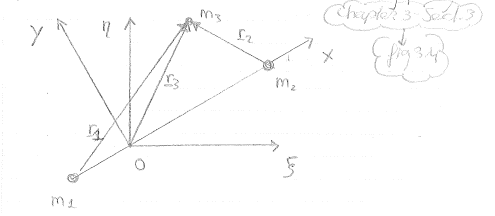
\includegraphics[width=0.5\columnwidth]{Figures/1a.png}
    \caption{Circular-restricted three body problem}
    \label{fig:3body}
\end{figure}

Parameters:\\
\begin{itemize}
    \item $x$ is the x-coordinate of body 3, so $x_3$
    \item $y$ is the y-coordinate of body 3, so $y_3$
    \item $r_1$ is the length of the position vector from body 1 to body 3
    \item $r_2$ is the length of the position vector from body 2 to body 3
    \item $\mu$ is the mass of body 2
    \item $1-\mu$ is the mass of body 1
    \item $C$ is the Jacobian Constant
\end{itemize}

The Surfaces of Hill are the surfaces in the XYZ-space on which the velocity of the third body is zero. This is the case when in equation \ref{eq:hill} V equals zero.

\subsection{1b}
\textit{Using clear sketches, provide a qualitative analysis of the shape and size of the Surfaces of Hill for changing values of C, and indicate the Lagrange points in the sketches.} \\

\begin{equation}\label{eq:hill2}
    r_3^2+\dfrac {2\left( 1-\mu \right) }{r_{1}}+\dfrac {2\mu }{r_{2}} = C
\end{equation}

If we look at the relevant equation, we can see that there for large values of C, there are 3 solutions:
\begin{enumerate}
    \item $r_3$ is very large, hence $p_3$ is far away from $p_1$ and $p_2$. The radius of the circle will be $\sqrt{C}$.
    \item $r_1$ is very small, hence $p_3$ is near $p_1$
    \item $r_2$ is very small, hence $p_3$ is near $p_2$
\end{enumerate}

When the value of C starts to decrease, we may observe three things. Either $r_3$ decreases, or $r_1$ increases, or $r_2$ increases. The resulting circles/ovals can be sketched in the XY-plane. We may find the Lagrange points at the points where the ovals intersect. This can be seen in the following figure:
\begin{figure}[H]
    \centering
    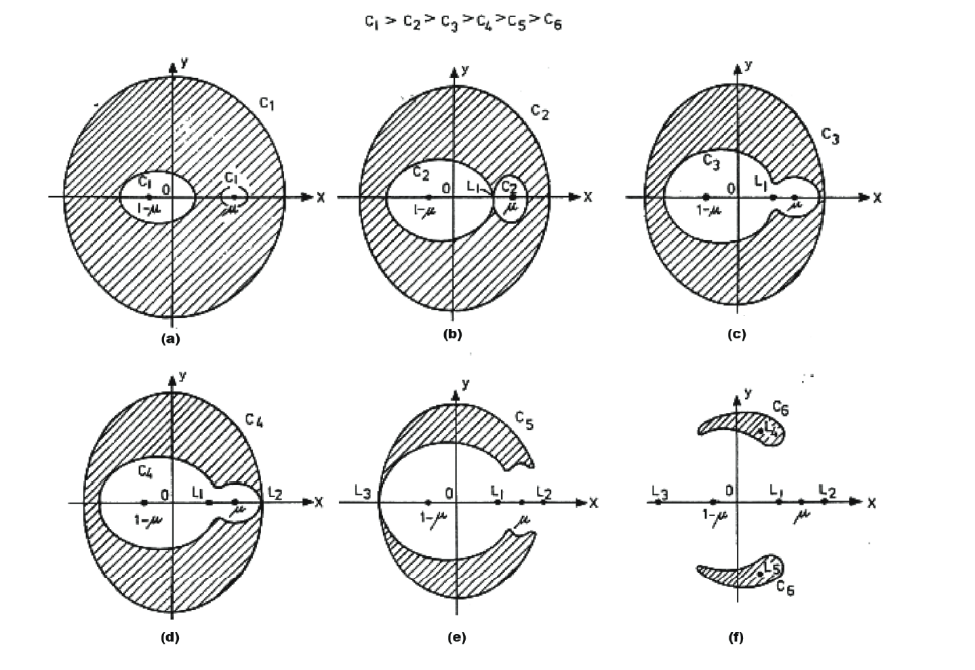
\includegraphics[width=1\columnwidth]{Figures/1b.png}
    \caption{Surfaces of Hill for various values of C}
    \label{fig:hill}
\end{figure}
The Lagrange point $L_1$ appears first, at the point where the ovals around $p_1$ and $p_2$ intersect. Next, $L_2$ and $L_3$ appear when the outer Surface of Hill intersects with the oval around $p_2$ and $p_1$ respectively. As C decreases further, it will look like Figure \ref{fig:hill}(f). The two leftover areas shrink until they vanish in points $L_4$ (above) and $L_5$ (below).


\subsection{1c}
\textit{Explain the physical interpretation of the Langrange points.} \\
The Lagrange points are those points where not only velocity V is zero, but the net acceleration is also zero. If body 3 were to be placed at such a point, without any residual velocity, it would remain at this point.



\subsection{1d}
\textit{It is possible to bring a spacecraft in a quasi-periodic "slowly changing elliptic" orbit around a Langrange point, also known as a Halo orbit. Give for all five Lagrange points a sketch of the orbit of a spacecraft around the point, and indicate the direction of motion of the vehicle.} \\

\begin{figure}[H]
    \centering
    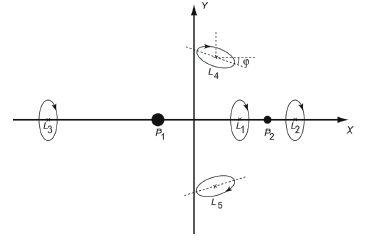
\includegraphics[width=0.7\columnwidth]{Figures/1d.png}
    \caption{Halo orbits around all five Lagrange points}
    \label{fig:haloes}
\end{figure}

In general, for a stable orbit around $L_4$ and $L_5$, $\phi$ is around 30 degrees.


\subsection{1e}
\textit{Provide an example of a possible application for such a Halo orbit.} \\
For missions to the far side of the moon, radio communication can be troublesome, as there is a moon in the way. A relay communication satellite around $L_2$ of the Earth-Moon system would solve this problem, as it is often able to see the far side of the moon and the Earth at the same time, provided the orbit radius is large enough.